% !TEX root = Dokumentation.tex
\section{Risikoanalyse}

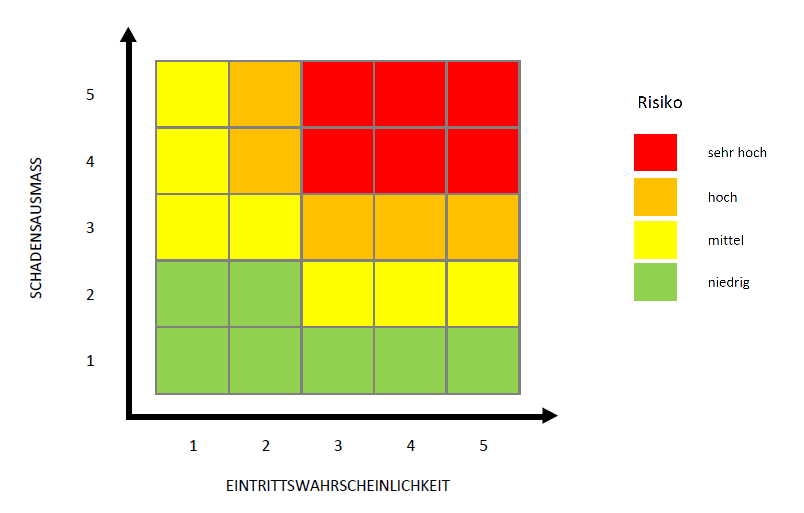
\includegraphics[width=0.8\textwidth]{Images/risikomatrix.png}

\subsection{Team}
\begin{table}[h]
\begin{tabular}{|p{3cm}|p{3cm}|p{3cm}|p{4cm}|}\hline
	
	\textbf{Risiko}	& 	\textbf{Wahrscheinlichkeit} & \textbf{Schadensausmass}  & \textbf{Massnahmen} \\\hline
	

	Mitglied verlässt das Team	&	1	&	4	&	Neuverteilung der Arbeiten \\\hline
	Unzuverlässigkeit eines Teammitglieds	&	2	&	3-4	&	 Absprache im Team, um eine Lösung zu finden  \\\hline
	Unstimmigkeiten unter den Teammitgliedern	& 	3	&	1-5	& Absprache im Team, um eine Lösung zu finden, evtl. auch Rat von Supervisor einholen.  \\\hline
\end{tabular}\\
\end{table}

\subsection{Projektmanagement}
\begin{table}[h]
\begin{tabular}{|p{3cm}|p{3cm}|p{3cm}|p{4cm}|}\hline
	
	\textbf{Risiko}	& 	\textbf{Wahrscheinlichkeit} & \textbf{Schadensausmass}  & \textbf{Massnahmen} \\\hline
		Missverständnisse bei den Anforderungen	&	3-4	&	3	& Absprache mit Supervisor  \\\hline
	Ineffizientes Arbeiten	&	3-4	&	2-3	& Neuorganisierung der Vorgehensweise  \\\hline
	
	Überschreitung des Budgets	&	1	&	4	& Absprache mit Supervisor  \\\hline
\end{tabular}\\
\end{table}

\subsection{Realisierung}
\begin{table}[h]
\begin{tabular}{|p{3cm}|p{3cm}|p{3cm}|p{4cm}|}\hline
	
	\textbf{Risiko}	& 	\textbf{Wahrscheinlichkeit} & \textbf{Schadensausmass}  & \textbf{Massnahmen} \\\hline
	
	Idee funktioniert nicht wie gewünscht	&	2	&	3-5	& neue Ideenfindung, Rat einholen  \\\hline
\end{tabular}\\
\end{table}

\subsection{Andere Risiken}
\begin{table}[h]
\begin{tabular}{|p{3cm}|p{3cm}|p{3cm}|p{4cm}|}\hline
	
	\textbf{Risiko}	& 	\textbf{Wahrscheinlichkeit} & \textbf{Schadensausmass}  & \textbf{Massnahmen} \\\hline
	
	Lange Lieferzeiten bei Bestellungen	&	3	&	2	& andere Arbeiten aufnehmen, früher bestellen  \\\hline
\end{tabular}\\
\end{table}

